% =====================================================================
% ARCHIVE (2026-10-06).  NOT input by main.tex.
% Material removed from the AISTATS draft when it was refocused on the
% application.  Each block records the file it came from.  The labels below
% are not defined in the paper and must not be referenced from it.
% =====================================================================

% ===== From sections/4.identifiability.tex: Sections 4.3 (Group Error at a Stated Noise Level), 4.4 (Uncertain Fingerprints), 4.5 (The IASA Procedure)
\subsection{Group Error at a Stated Noise Level}
\label{subsec:group_error}

Exact identifiability does not bound the error of a group's signal; the distance
between the group's span and the span of everything else does.

\begin{definition}[Separation]
\label{def:separation}
The \emph{separation} of \(g\subseteq E\) is \(s_g=\sin\theta_g\), where
\(\theta_g\) is the smallest principal angle \citep{bjorck1973numerical} between
\(\operatorname{col}(\At_g)\) and \(\operatorname{col}(\At_{E\setminus g})\), with
\(s_g=1\) when either space is \(\{0\}\).
\end{definition}

\(s_g\) depends only on \(g\) and its complement, and \(s_g>0\) for every block of an
identifiable partition.  For two components, \(s=\sqrt{1-\rho^2}\), where
\(\rho=|\at_1^\top\at_2|/(\|\at_1\|_2\|\at_2\|_2)\) is their coherence; for a single
component, \(1/s_j^2\) is the uncentered variance-inflation factor of column \(j\).

\begin{theorem}[Group-signal error]
\label{thm:group_error}
Let \(\mathcal P\) be identifiable and let \(\widehat{\mathbf c}\) be any
least-squares solution, or any NNLS solution with \(\mathbf c\ge0\).
\begin{enumerate}[label=(\alph*),leftmargin=*,itemsep=0pt,topsep=2pt]
  \item The group signals \(\At_g\widehat{\mathbf c}_g\) do not depend on which
  solution is chosen, and for every \(g\in\mathcal P\),
  \begin{equation}
  \|\At_g(\widehat{\mathbf c}_g-\mathbf c_g)\|_2
  \le
  \frac{\|P_{\At}\widetilde{\boldsymbol\epsilon}\|_2}{s_g}.
  \label{eq:group_bound}
  \end{equation}
  \item If \(\widetilde{\boldsymbol\epsilon}=P_Q^\perp\boldsymbol\epsilon\) with
  \(\boldsymbol\epsilon\sim N(0,\sigma^2 I_N)\) and \(\widehat{\mathbf c}\) is a
  least-squares solution, then with \(r_g=\operatorname{rank}(\At_g)\),
  \(\mathbb E\|\At_g(\widehat{\mathbf c}_g-\mathbf c_g)\|_2^2\le\sigma^2r_g/s_g^2\),
  with equality when \(r_g=1\), and with probability at least \(1-\delta\),
  \begin{equation}
  \|\At_g(\widehat{\mathbf c}_g-\mathbf c_g)\|_2
  \le
  \frac{\sigma\bigl(\sqrt{r_g}+\sqrt{2\log(1/\delta)}\bigr)}{s_g}.
  \label{eq:group_bound_gauss}
  \end{equation}
\end{enumerate}
\end{theorem}

The bound does not contain \(\sigma_J(\At)\): columns inside a group can be nearly or
exactly dependent, which makes the coefficient error of
Proposition~\ref{prop:noise_robust} arbitrarily large, while the group's signal error
stays fixed (Section~\ref{subsec:synthetic_study}).  For a single component, (b) is
the classical formula \(\|\at_j\|^2\operatorname{Var}(\widehat c_j)=\sigma^2/s_j^2\).

\begin{definition}[Reportable partition]
\label{def:reportable}
An identifiable partition is \emph{reportable at threshold \(\tau_\theta\in(0,1]\)}
if \(s_g\ge\tau_\theta\) for every block.
\end{definition}

By~\eqref{eq:group_bound_gauss} and Corollary~\ref{cor:uniform_bound}, \(\tau_\theta\) is chosen from the noise level and a
tolerance on the group-signal error.  Our default, \(\tau_\theta=\sqrt{1-0.99^2}\approx
0.141\), reproduces a pairwise coherence threshold of \(0.99\) when \(J=2\).

\begin{proposition}[Structure of reportable partitions]
\label{prop:reportable_structure}
\leavevmode
\begin{enumerate}[label=(\alph*),leftmargin=*,itemsep=0pt,topsep=2pt]
  \item The one-block partition \(\{E\}\) is reportable at every \(\tau_\theta\).
  \item If \(g\) and \(h\) are blocks of an identifiable partition, then
  \(1/s_{g\cup h}\le1/s_g+1/s_h\), and reportable partitions are not closed under
  coarsening.
  \item Minimal reportable partitions need not be unique.
\end{enumerate}
\end{proposition}

A procedure must therefore say which reportable partition it returns.  IASA takes the
blocks of \(\mathcal P^\star\vee\mathcal D\) as \emph{atoms}.  With \(q\le12\) atoms it finds
the minimal reportable partition with the most blocks by dynamic programming over unions
of atoms in \(O(3^q)\) time, breaks ties by the largest smallest separation, and lists any
remaining ties; with more atoms it merges atoms greedily, without an optimality guarantee
(Appendix~\ref{app:identifiability_proofs}).

\begin{proposition}[Stability under operator error]
\label{prop:grouping_stability}
Let \(\At'=\At+\Delta\).  For \(S\subseteq E\) with \(\At_S\) of full column rank and
\(\|\Delta_S\|_2\le\sigma_{\min}(\At_S)/2\), let
\(\beta_S=\arcsin\bigl(\|\Delta_S\|_2/(\sigma_{\min}(\At_S)-\|\Delta_S\|_2)\bigr)\).
If this holds for \(S=g\) and \(S=E\setminus g\), with \(g\) nonempty and proper, then
\(|\theta_g(\At')-\theta_g(\At)|\le\beta_g+\beta_{E\setminus g}\).  If \(\At\) has full
column rank, \(\|\Delta\|_2\le\sigma_J(\At)/2\), and
\(|\theta_g(\At)-\arcsin\tau_\theta|>\beta_g+\beta_{E\setminus g}\) for every nonempty
proper union \(g\) of atoms, the reportable partitions of \(\At'\) and \(\At\) coincide,
and so do the minimal reportable partitions.
\end{proposition}

\subsection{Uncertain Fingerprints}
\label{subsec:uncertain_fingerprints}

The operator is itself estimated, for example from a transport model driven by an
estimated wind field: \(\At=\At^\star+\Delta\), where \(\At^\star\) holds the latent
fingerprints.  The grouping of interest is the \emph{latent grouping} \(\mathcal L\),
the finest identifiable partition of \(\At^\star\).  Exact rank computations on
\(\At\) cannot return it, because \(\Delta\) makes \(\At\) full rank in general.  Let
\(\operatorname{rank}_\tau(M)\) be the number of singular values of \(M\) above
\(\tau\), and call \(\mathcal P\) \emph{\(\tau\)-identifiable} for \(\At\) if
\(\sum_{g\in\mathcal P}\operatorname{rank}_\tau(\At_g)=\operatorname{rank}_\tau(\At)\).

\begin{theorem}[Recovery of the latent grouping]
\label{thm:latent_recovery}
Suppose \(\|\Delta\|_2<\tau\) and, for every \(S\subseteq E\), every singular value of
\(\At^\star_S\) is either \(0\) or larger than \(\tau+\|\Delta\|_2\).  Then a partition is
\(\tau\)-identifiable for \(\At\) if and only if it is identifiable for \(\At^\star\).  In
particular the \(\tau\)-identifiable partitions of \(\At\) have a unique finest element,
equal to \(\mathcal L\).
\end{theorem}

If \(\Delta=P_Q^\perp\Delta_0\) and \(\Delta_0\) has independent \(N(0,\sigma_f^2)\)
entries, then \(\|\Delta\|_2\le\sigma_f(\sqrt N+\sqrt J+t)\) with probability at least
\(1-2e^{-t^2/2}\) \citep[Corollary~5.35]{vershynin2012introduction}, which sets
\(\tau\); \(\sigma_f\) comes from the spread of an operator ensemble.  Without the
margin condition there can be several minimal \(\tau\)-identifiable partitions.  IASA
then returns the one with the smallest largest discarded singular value
\(D(\mathcal P)=\max_{g\in\mathcal P}\sigma_{k_g+1}(\At_g)\), with
\(k_g=\operatorname{rank}_\tau(\At_g)\).  Appendix~\ref{app:identifiability_proofs}
converts \(D(\mathcal P)\) into a Gaussian p-value for the hypothesis that \(\mathcal P\)
is identifiable for \(\At^\star\) and every nonzero singular value of every block
\(\At^\star_g\) is at least \(2\tau\); the rule's choice, the smallest \(D(\mathcal P)\), has the largest p-value, and
\(D\) separates candidates tied at p-value \(1\).

\begin{proposition}[Choosing the latent grouping]
\label{prop:latent_tiebreak}
Suppose \(\|\Delta\|_2<\tau\) and the nonzero singular values of \(\At^\star\), and of
\(\At^\star_S\) for every \(S\) contained in a block of \(\mathcal L\), exceed
\(\tau+\|\Delta\|_2\).  Then \(\mathcal L\) is a minimal \(\tau\)-identifiable
partition of \(\At\).  Let \(d_\star\) be the minimum of
\(\max_{g\in\mathcal P}\sigma_{k_g+1}(\At^\star_g)\) over all partitions \(\mathcal P\)
that are not coarsenings of \(\mathcal L\) and all integers \(0\le k_g\le|g|\) with
\(\sum_gk_g=\operatorname{rank}(\At^\star)\).  Then \(d_\star>0\), and if
\(\|\Delta\|_2<d_\star/2\) the rule returns \(\mathcal L\).  Under the Gaussian model, if
\(b=\sigma_f(\sqrt N+\sqrt J+t)\) satisfies \(b<\min(\tau,d_\star/2)\) and the
nonzero singular values above exceed \(\tau+b\), the rule returns \(\mathcal L\) with
probability at least \(1-2e^{-t^2/2}\).
\end{proposition}

When \(\mathcal L\) consists of single components but some nonzero singular value of \(\At^\star\) is at most \(\tau+\|\Delta\|_2\), the candidates are coarser than \(\mathcal L\) and the choice among them is a reporting decision.  The reporting guarantee does not depend on
that choice:

\begin{corollary}[Uniform reporting bound]
\label{cor:uniform_bound}
Under the noise model of Theorem~\ref{thm:group_error}(b), with probability at least
\(1-\delta\), for every identifiable partition of \(\At\), every block \(g\), the
least-squares estimate and, when \(\mathbf c\ge0\), the NNLS estimate,
\(\|\At_g(\widehat{\mathbf c}_g-\mathbf c_g)\|_2\le
\sigma\bigl(\sqrt{\operatorname{rank}(\At)}+\sqrt{2\log(1/\delta)}\bigr)/s_g\).  If
\(\boldsymbol\epsilon\sim N(0,\Sigma)\), the same holds with \(\sigma^2\) replaced by
\(\|\Sigma\|_2\).
\end{corollary}

The partition may therefore be chosen by any rule, including one that uses the data;
operator error enters as additional observation noise
(Proposition~\ref{prop:operator_perturbation}).

\subsection{The IASA Procedure}
\label{sec:identifiability_aware_method}

\noindent\textbf{Diagnostics.}
IASA reports a fixed panel of diagnostics computed from \(\At\), each with a
threshold declared before fitting (Appendix~\ref{app:diagnostics_definitions},
Table~\ref{tab:thresholds}): the numerical rank at tolerance \(\tau_{\mathrm{num}}\);
the smallest singular value \(\sigma_J\), padded with zeros when \(J>N\) or \(\At\) is
rank deficient; the condition number \(\kappa=\sigma_1/\sigma_J\); the effective rank
\(r_{\mathrm{eff}}(\tau_\sigma)\), the number of singular values above a noise-derived
threshold \(\tau_\sigma\); the visibility \(v_j=\|\at_j\|_2\) and the weak set
\(\mathcal W=\{j:v_j\le\tau_v\}\); the nuisance absorption
\(a_j=\|P_Q\mathbf a_j\|_2/\|\mathbf a_j\|_2\); the pairwise coherences \(\rho_{ij}\) (\(\rho\) above, for columns \(i\) and \(j\));
and the separations \(s_g\) of the reported blocks.

\begin{algorithm}[t]
\caption{Identifiability-Aware Source Attribution (IASA)}
\label{alg:iasa}
\footnotesize
\begin{algsteps}
  \item \textbf{Declare} \(Q\), the components, \(\mathcal D\), the fixed-zero set
  \(\mathcal F_0\) and all thresholds before inspecting any fit.
  \item \textbf{Operator:} build \(A(\omega)\) from the context (application: wind
  field, lagged transport response, lag chosen from operator geometry;
  Appendix~\ref{app:application}).
  \item \textbf{Align and project:} remove unobserved rows identically from
  \(\mathbf y\), \(A(\omega)\) and \(Q\); form \(\yt\) and \(\At\)
  \eqref{eq:projected_model}.
  \item \textbf{Diagnose:} singular values, numerical rank, \(r_{\mathrm{eff}}\),
  visibility, absorption, coherence; weak set \(\mathcal W\).
  \item \textbf{Group:} \(\mathcal P^\star\) at \(\tau_{\mathrm{num}}\)
  (Theorem~\ref{thm:groupings}c), or the estimated latent grouping at \(\tau\) when an
  operator ensemble gives \(\sigma_f\); atoms: its join with \(\mathcal D\); reported
  partition at \(\tau_\theta\).
  \item \textbf{Fit:} solve \eqref{eq:nnls_estimator}; form the group signals
  \(\At_g\widehat{\mathbf c}_g\) and their \(L_1\) shares.
  \item \textbf{Adequacy:} parametric-bootstrap residual test if a calibrated noise
  model exists; otherwise label the residual summary uncalibrated.
  \item \textbf{Report} group signals and shares, singleton coefficients,
  uncertainty, robustness scenarios, adequacy, diagnostics, separations and ties.
\end{algsteps}
\end{algorithm}

Algorithm~\ref{alg:iasa} combines the estimator~\eqref{eq:nnls_estimator}, the
diagnostics and the grouping.  All declarations and thresholds precede the fit, and
the grouping uses \(\At\) only, so it is fixed before \(\widehat{\mathbf c}\) exists.
Problem~\eqref{eq:nnls_estimator} is solved by projected FISTA \citep{beck2009fast}
(Appendix~\ref{app:pytorch_solver}).

\noindent\textbf{Uncertainty and adequacy.}
IASA reports an active-set ridge covariance of the fitted contributions, the
least-squares group-signal covariance from the proof of Theorem~\ref{thm:group_error}(b) and the bound
of Corollary~\ref{cor:uniform_bound} when a noise level is declared, and quantiles across operator-ensemble refits; operator uncertainty and
robustness scenarios are never pooled.  With an externally calibrated noise model, a
nuisance-orthogonal residual statistic is calibrated by a parametric bootstrap with
refitting; otherwise residual summaries are labelled uncalibrated
(Appendix~\ref{app:reporting_details}).

% ===== sections/5.experiments.tex (Section 5, Synthetic Experiments), whole file
\section{Synthetic Experiments}
\label{sec:experiments}

\subsection{Synthetic Study}
\label{subsec:synthetic_study}

\noindent\textbf{Setup.}
Planted operators have blocks of columns whose spans are drawn at random inside an
ambient space slightly larger than the sum of their dimensions and embedded in
\(\mathbb R^N\); a random nuisance basis of dimension \(5\) is projected out, and
\(\mathbf c\sim\mathrm{Unif}[0.5,1.5]^J\).  Inside a block the columns are exactly
dependent (\(k\) columns in general position in \(k-1\) dimensions, so no pair is
nearly parallel) or nearly dependent with spread \(\xi\), which makes the block's
smallest singular value proportional to \(\xi\) without changing its span.  Noise is
Gaussian (Appendix~\ref{app:synthetic_details}).

\begin{figure*}[t]
\centering
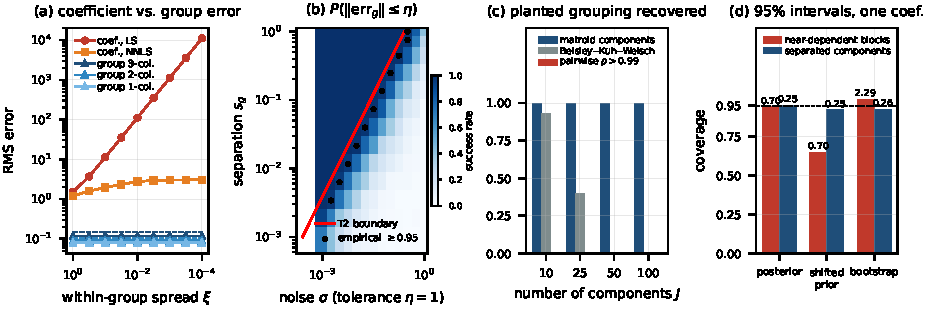
\includegraphics[width=\textwidth]{figures/fig_synthetic.pdf}
\caption{Synthetic study.  \textbf{(a)}~Least-squares coefficient error and
group-signal error (triangles) against the within-block spread \(\xi\), with the
Theorem~\ref{thm:group_error} value \(\sigma\sqrt{r_g}/s_g\) (dashed).
\textbf{(b)}~Fraction of draws with group-signal error at most \(\eta=1\); red: boundary
of~\eqref{eq:group_bound_gauss} at \(\delta=0.05\); black: observed boundary.
\textbf{(c)}~Rate at which each rule returns the planted partition.
\textbf{(d)}~Coverage of nominal \(95\%\) intervals for single coefficients; numbers
are median widths.}
\label{fig:synthetic}
\end{figure*}

\noindent\textbf{The finest identifiable partition.}
With exactly dependent blocks of \(1\)--\(5\) columns, the matroid components of
Theorem~\ref{thm:groupings} return the planted partition in all \(30\) operators at
each of \(J=10,25,50,100\), in \(0.4\) to \(55\) ms (Figure~\ref{fig:synthetic}(c)).  A
pairwise rule with \(\rho_{ij}>0.99\) returns it in none, because it splits
\(99\)--\(100\%\) of the blocks with three or more columns, whose pairwise
coherences are moderate.  The Belsley--Kuh--Welsch collinearity sets \citep{belsley1980regression}
(condition index above \(30\), variance-decomposition proportion above \(0.5\))
return it in \(93\%\), \(40\%\), \(0\%\) and \(0\%\) of operators.

\noindent\textbf{Group error does not depend on within-group conditioning.}
In Figure~\ref{fig:synthetic}(a) (blocks of \(3\), \(2\) and \(1\) columns, \(N=200\),
\(\sigma=0.05\)), \(\sigma_J(\At)\) falls from \(3.5\times10^{-2}\) to
\(4.6\times10^{-6}\) as \(\xi\) falls from \(1\) to \(10^{-4}\), and the least-squares
coefficient error rises in proportion, from \(1.5\) to \(1.1\times10^4\) (NNLS: \(1.2\)
to \(3.0\)).  The least-squares group-signal errors are the same at every \(\xi\):
\(0.118\), \(0.089\) and \(0.080\) for the 3-, 2- and 1-column blocks, against the
Theorem~\ref{thm:group_error} values \(0.147\), \(0.104\) and \(0.078\); the
single-column block attains its value up to Monte Carlo error, as the equality case
predicts.  NNLS group errors are \(0.050\)--\(0.113\).

\noindent\textbf{The noise-level boundary.}
In Figure~\ref{fig:synthetic}(b) (two 2-column blocks, \(200\) draws per cell), no
cell with \(\sigma\) below the boundary of~\eqref{eq:group_bound_gauss} has a success
fraction below \(0.95\).  The observed boundary lies at \(1.2\)--\(2.0\) times the
predicted noise level over three decades of separation.

\noindent\textbf{Grouping procedure and operator error.}
The greedy rule returns a minimal reportable partition in \(98\)--\(100\%\) of
operators with one to three planted near-dependencies at \(J=6,8,10\), and more than
one minimal reportable partition exists in \(0\)--\(6.7\%\) of them.  Over \(1000\)
random operator perturbations the bound of Proposition~\ref{prop:grouping_stability}
held in all \(115{,}688\) block checks, and the reported partition never changed when
every margin exceeded its bound (Appendix~\ref{app:synthetic_details}).

\subsection{Statistical Baselines}
\label{subsec:statistical_baselines}

On \(40\) operators with blocks of \(4\), \(3\), \(1\) and \(1\) columns, nearly
dependent inside blocks (\(\xi=10^{-3}\), median largest within-block coherence
\(0.97\)), \(N=200\) and \(\sigma=0.05\), the separation rule at \(\tau_\theta=0.141\)
returns the planted partition for all \(40\) operators, the Belsley--Kuh--Welsch sets
for \(75\%\), and the pairwise rule and the exact components at
\(\tau_{\mathrm{num}}\) for none.  The median largest NNLS group-signal error at each
rule's partition, divided by the norm of the total projected signal, is \(0.040\),
\(0.041\), \(1.13\) and \(2.46\) respectively: the two rules that split near-dependent
columns report group signals whose errors exceed the total signal.  At the planted
partition, NNLS, ridge with generalized cross-validation \citep{golub1979generalized}
and truncated SVD \citep{hansen1987truncated} have median relative group-signal errors
\(0.054\), \(0.055\) and \(0.058\).  Ridge reports every coefficient without indicating
which are determined, and only \(9\%\) of the retained truncated-SVD directions have
at least \(90\%\) of their weight on one block.

\noindent\textbf{Intervals for single coefficients} (Figure~\ref{fig:synthetic}(d)).
A Gaussian posterior with a prior that matches the distribution that generated
\(\mathbf c\) covers \(94\%\) of coefficients in near-dependent blocks; with the prior
mean moved by \(\pm0.5\), coverage falls to \(65\%\) at the same median width
(\(0.70\)), because the posterior in directions the data do not determine is the
prior.  Residual-bootstrap NNLS intervals cover \(99\%\) but are \(9\) times wider than
for separated components.  Neither method states which quantities the data determine.

% ===== sections/D0.synthetic.tex (Appendix: Synthetic Study Details), whole file
\section{Synthetic Study: Details}
\label{app:synthetic_details}

\noindent\textbf{Generator.}  For block sizes \(k_1,\dots,k_m\), block \(g\) has
coordinates \(W_g\in\mathbb R^{r_g\times k_g}\) with unit-norm columns: one column
(\(k_g=1\)); \(k_g\) Gaussian columns in \(r_g=k_g-1\) dimensions (\emph{exact}); the
same with an extra coordinate of size \(\xi\) (\emph{near circuit},
\(r_g=k_g\)); or a common first coordinate with spread \(\xi\) in the others
(\emph{near}, \(r_g=k_g\)).  Each block's subspace is a random \(r_g\)-dimensional
subspace of \(\mathbb R^D\), \(D=\sum_gr_g+\text{slack}\), embedded in \(\mathbb R^N\)
by a random orthonormal map, and its columns are the embedded subspace basis times
\(W_g\).  Columns are permuted at random.  A Gaussian nuisance basis \(Q\) with five
columns is projected out of the operator and of
\(\mathbf y=A\mathbf c+Q\boldsymbol\gamma+\boldsymbol\epsilon\), with
\(\mathbf c\sim\mathrm{Unif}[0.5,1.5]^J\), \(\boldsymbol\gamma\sim N(0,I)\) and
\(\boldsymbol\epsilon\sim N(0,\sigma^2I_N)\).

\noindent\textbf{Settings.}
\begin{itemize}[leftmargin=*,itemsep=0pt,topsep=2pt]
  \item \emph{Exact recovery} (Figure~\ref{fig:synthetic}(c)): \(N=300\), slack \(5\),
  block sizes drawn uniformly from \(1\)--\(5\) until \(J\) is reached, exact blocks,
  \(30\) operators per \(J\in\{10,25,50,100\}\).  Matroid components at
  \(\tau_{\mathrm{num}}\); pairwise rule \(\rho_{ij}>0.99\); Belsley--Kuh--Welsch sets
  with unit-length columns, condition index above \(30\) and variance-decomposition
  proportion above \(0.5\), overlapping sets merged.
  \item \emph{Within-block conditioning} (Figure~\ref{fig:synthetic}(a)): blocks of
  \(3\), \(2\), \(1\) columns, near blocks, slack \(2\), \(N=200\), \(\sigma=0.05\);
  \(\xi\in\{10^0,10^{-0.5},\dots,10^{-4}\}\) with the same subspaces at every
  \(\xi\); \(2000\) draws per \(\xi\).  The plotted bound is the root-mean-square
  form \(\sigma\sqrt{r_g}/s_g\) of Theorem~\ref{thm:group_error}(b).
  \item \emph{Phase diagram} (Figure~\ref{fig:synthetic}(b)): two 2-column blocks
  spanning \(\operatorname{span}(\mathbf e_1,\mathbf e_2)\) and
  \(\operatorname{span}(\cos\theta\,\mathbf e_1+\sin\theta\,\mathbf e_3,\mathbf e_4)\),
  embedded in \(\mathbb R^{100}\), each with coordinates \(((1,0),(0.6,0.8))\), so
  \(s_g=\sin\theta\); \(\mathbf c=(1,0.7,0.9,1.2)\); \(13\) values of \(\theta\)
  log-spaced in \([10^{-3},\pi/2]\) and \(13\) values of \(\sigma\) log-spaced in
  \([10^{-3},1]\); \(200\) least-squares fits per cell; success means
  \(\|\At_g(\widehat{\mathbf c}_g-\mathbf c_g)\|_2\le\eta=1\) for the first block.
  The predicted boundary is \(\sigma=\eta s_g/(\sqrt2+\sqrt{2\log20})\).
  \item \emph{Exhaustive and greedy}: \(N=50\), Gaussian columns with one to three
  planted near-dependencies \(\mathbf a_k=w_1\mathbf a_i+w_2\mathbf a_j+0.1\mathbf z\),
  \(\tau_\theta=0.2\), \(60\) operators per \(J\in\{6,8,10\}\).
  \item \emph{Operator error}: blocks of \(3,2,1,1\) columns, near blocks with
  \(\xi=0.3\), slack \(1\), \(N=200\); \(40\) operators with \(25\) Gaussian perturbations
  each, scaled to \(\|\Delta\|_2=10^u\|\At\|_2\) with \(u\sim\mathrm{Unif}[-4,-1]\); the
  bound is checked on all \(126\) nonempty proper subsets, at
  \(\tau_\theta=\sqrt{1-0.99^2}\).
  \item \emph{Baselines} (Section~\ref{subsec:statistical_baselines}): blocks of
  \(4,3,1,1\) columns, near-circuit blocks with \(\xi=10^{-3}\), slack \(4\),
  \(N=200\), \(\sigma=0.05\); \(40\) operators with \(40\) draws each.  Ridge with
  \(\lambda\) chosen by generalized cross-validation over \(41\) values log-spaced in
  \([10^{-8},10^2]\sigma_1^2\) \citep{hoerl1970ridge,golub1979generalized}; truncated
  SVD with the rank chosen by generalized cross-validation \citep{hansen1987truncated};
  Gaussian posterior with prior \(N(\boldsymbol\mu_0,0.29^2I)\), where
  \(\boldsymbol\mu_0=\mathbf 1\) or \(\boldsymbol\mu_0=\mathbf 1\pm0.5\) with signs drawn
  once per operator, and the true \(\sigma\); residual bootstrap with \(200\) resamples
  of the centered NNLS residuals and percentile intervals
  \citep{efron1993introduction}.  Intervals are evaluated on eight draws per operator.
\end{itemize}

\noindent\textbf{Results not shown in the main text.}  At \(\tau_\theta=0.2\), the greedy
rule returned a minimal reportable partition in \(100\%\), \(100\%\) and \(98\%\) of the
\(60\) operators at \(J=6,8,10\), with on average \(99.7\%\) of the maximum number of blocks
at \(J=10\); exhaustive enumeration took \(0.9\), \(4.1\) and \(19.6\) ms.  More than one
minimal reportable partition existed in \(6.7\%\), \(0\%\) and \(3.3\%\) of these operators.
Under operator error, every margin exceeded its bound in \(235\) of the \(1000\)
perturbations and the reported partition never changed in those; all \(198\) changes of
the reported partition occurred with some margin within its bound.

\noindent\textbf{Code and run time.}  The study is
\texttt{experiments/iasa\_synthetic/run\_study.py} with seed \(20261004\) (plus the
index of each part); results are in \texttt{evaluation/iasa\_synthetic/results.json}.
The six parts take \(2.2\), \(1.1\), \(0.4\), \(1.7\), \(13.8\) and \(2.4\) seconds on one
laptop CPU (Apple M5).

\noindent\textbf{Latent grouping under operator error.}  Latent fingerprints
\(\boldsymbol\mu_0\), \(\boldsymbol\mu_2=1.3\boldsymbol\mu_0\) (exactly dependent),
\(\boldsymbol\mu_1\) at an angle drawn uniformly from \([0.02,0.4]\) from both, and a
separate \(\boldsymbol\mu_3\), in \(\mathbb R^{10}\), so \(\mathcal L=\{\{0,2\},\{1\},\{3\}\}\);
operator error with independent \(N(0,\sigma_f^2)\) entries, \(\sigma_f\) log-uniform in
\([10^{-3.5},10^{-1.3}]\); \(\tau=\sigma_f(\sqrt{10}+2+u)\) with \(u\sim\mathrm{Unif}[1,6]\);
\(6000\) instances.  \(\mathcal L\) was the only minimal \(\tau\)-identifiable partition in
\(4622\) instances.  In \(242\) instances \(\mathcal L\) and at least one competitor were
both minimal; the inequalities of the proof of Proposition~\ref{prop:latent_tiebreak}
(\(D(\mathcal L)\le\|\Delta\|_2\), \(d_{\mathcal P}>0\),
\(D(\mathcal P)\ge d_{\mathcal P}-\|\Delta\|_2\)) held in all \(242\), the condition
\(\|\Delta\|_2<d_{\mathcal P}/2\) for every competitor held in \(54\), and the rule
returned \(\mathcal L\) in all \(242\) (study part \texttt{e1f}).

% ===== From sections/A.proofs.tex: An Oblique Projection Lemma
\subsection{An Oblique Projection Lemma}

\begin{lemma}
\label{lem:oblique}
Let \(U=V\oplus W\) with \(V\ne\{0\}\ne W\), let \(\theta\in(0,\pi/2]\) be the smallest
principal angle between \(V\) and \(W\), and let \(\pi\) be the projection onto
\(V\) along \(W\), defined on \(U\).  Then \(\|\pi\|_2=1/\sin\theta\).
\end{lemma}

\begin{proof}
Write \(\mathbf u=\mathbf x+\mathbf w\) with \(\mathbf x\in V\), \(\mathbf w\in W\).
By the definition of \(\theta\),
\(|\mathbf x^\top\mathbf w|\le\cos\theta\,\|\mathbf x\|_2\|\mathbf w\|_2\), so
\[
\|\mathbf u\|_2^2\ge\|\mathbf x\|_2^2+\|\mathbf w\|_2^2
-2\cos\theta\|\mathbf x\|_2\|\mathbf w\|_2
=(\|\mathbf w\|_2-\cos\theta\|\mathbf x\|_2)^2+\sin^2\theta\|\mathbf x\|_2^2
\ge\sin^2\theta\|\mathbf x\|_2^2 ,
\]
which gives \(\|\pi\mathbf u\|_2\le\|\mathbf u\|_2/\sin\theta\).  For unit principal
vectors \(\mathbf x_0\in V\), \(\mathbf w_0\in W\) with
\(\mathbf x_0^\top\mathbf w_0=\cos\theta\), the vector
\(\mathbf u=\mathbf x_0-\cos\theta\,\mathbf w_0\) has \(\|\mathbf u\|_2=\sin\theta\)
and \(\pi\mathbf u=\mathbf x_0\), so the bound is attained
\citep{ipsen1995angle}.
\end{proof}

If \(V=\{0\}\), then \(\pi=0\); if \(W=\{0\}\), \(\pi\) is the identity on \(U\).  Both
cases are consistent with the convention \(s_g=1\).

% ===== From sections/A.proofs.tex: Group-Signal Error, Uncertain Fingerprints, A Ridge Penalty
\subsection{Group-Signal Error}

\noindent\textbf{Proof of Theorem~\ref{thm:group_error}.}
\emph{(a)}  By Theorem~\ref{thm:groupings}(a), \(U=\bigoplus_{g}V_g\), and
\(W_g=\bigoplus_{h\ne g}V_h\).  Let \(\pi_g\) be the projection of \(U\) onto
\(V_g\) along \(W_g\).  For any \(\mathbf z\),
\(A\mathbf z=\sum_gA_g\mathbf z_g\) with \(A_g\mathbf z_g\in V_g\), so
\(A_g\mathbf z_g=\pi_g(A\mathbf z)\).  All least-squares solutions have the fitted
signal \(P_A\yt\), and all NNLS solutions have the fitted signal \(\Pi_C(\yt)\),
which is unique because \(C\) is closed and convex; hence the group signals do not
depend on the solution.  Moreover
\(A_g(\widehat{\mathbf c}_g-\mathbf c_g)=\pi_g\bigl(A(\widehat{\mathbf c}-\mathbf c)\bigr)\),
where \(A(\widehat{\mathbf c}-\mathbf c)=P_A\widetilde{\boldsymbol\epsilon}\) for
least squares and \(\|A(\widehat{\mathbf c}-\mathbf c)\|_2\le
\|P_A\widetilde{\boldsymbol\epsilon}\|_2\) for NNLS (proof of
Proposition~\ref{prop:noise_robust}).  Lemma~\ref{lem:oblique} with \(V=V_g\),
\(W=W_g\) gives \(\|\pi_g\|_2\le1/s_g\), with equality when \(V_g\) and \(W_g\) are
nonzero, which proves~\eqref{eq:group_bound}.

\emph{(b)}  Since \(U\subseteq\operatorname{col}(Q)^\perp\),
\(P_A\widetilde{\boldsymbol\epsilon}=P_AP_Q^\perp\boldsymbol\epsilon
=P_A\boldsymbol\epsilon\).  The least-squares error of block \(g\) is
\(M\boldsymbol\epsilon\) with \(M=\pi_gP_A\), a matrix of rank \(r_g\) with
\(\|M\|_2=\|\pi_g\|_2=1/s_g\) when \(r_g\ge1\); when \(r_g=0\), \(M=0\) and the
error is zero.  Hence
\(\mathbb E\|M\boldsymbol\epsilon\|_2^2=\sigma^2\|M\|_F^2\le\sigma^2r_g\|M\|_2^2
=\sigma^2r_g/s_g^2\), with equality when \(r_g=1\) because \(M\) then has one nonzero
singular value.  The map \(\boldsymbol\epsilon\mapsto\|M\boldsymbol\epsilon\|_2\) is
\(\|M\|_2\)-Lipschitz, so the Gaussian concentration inequality of
Tsirelson, Ibragimov and Sudakov \citep{boucheron2013concentration} gives
\(\|M\boldsymbol\epsilon\|_2\le\mathbb E\|M\boldsymbol\epsilon\|_2
+\sigma\|M\|_2\sqrt{2\log(1/\delta)}\) with probability at least \(1-\delta\), and
\(\mathbb E\|M\boldsymbol\epsilon\|_2\le\sigma\|M\|_F\le\sigma\sqrt{r_g}/s_g\).
\(\square\)

\noindent\textbf{Proof of Proposition~\ref{prop:reportable_structure}.}
\emph{(a)}  \(\{E\}\) is identifiable and \(s_E=1\) by convention.
\emph{(b)}  With \(\pi_g\) as above, \(\pi_{g\cup h}=\pi_g+\pi_h\), because both send
\(\sum_k\mathbf x_k\) (with \(\mathbf x_k\in V_k\)) to \(\mathbf x_g+\mathbf x_h\).  By
Lemma~\ref{lem:oblique},
\(1/s_{g\cup h}=\|\pi_g+\pi_h\|_2\le1/s_g+1/s_h\) when \(V_{g\cup h}\ne\{0\}\); when
\(V_{g\cup h}=\{0\}\), \(s_{g\cup h}=1\) and the inequality holds because
\(1/s_g,1/s_h\ge1\).  For the \(4\times4\) operator
\[
\begin{pmatrix}
0.248&-0.142&0.165&0.828\\
0.899&-0.775&-0.917&0.229\\
-0.356&-0.381&0.243&-0.507\\
-0.063&-0.484&-0.270&0.069
\end{pmatrix}
\]
the four singletons have separations of at least \(0.3\), while the blocks of
\(\{\{1,2\},\{3,4\}\}\) have separation below \(0.3\), so at \(\tau_\theta=0.3\) a
reportable partition has a coarsening that is not reportable.
\emph{(c)}  Let \(\at_1=(1,0,0)\), \(\at_2=(\cos a,\sin a,0)\) and
\(\at_3=(\cos a,0,\sin a)\) with \(a=0.3\), and \(\tau_\theta=0.25\).
\(\operatorname{span}(\at_1,\at_2)\) is the plane \(x_3=0\), at angle
\(a\) from \(\at_3\), so both blocks of \(\{\{1,2\},\{3\}\}\) have separation
\(\sin a=0.296\); by symmetry so do those of \(\{\{1,3\},\{2\}\}\).  The angle
between \(\at_1\) and \(\operatorname{span}(\at_2,\at_3)\) has sine
\(\sin a/\sqrt{1+\cos^2a}=0.214\), which is \(s_1\) and also the separation of
\(\{2,3\}\).  At \(\tau_\theta=0.25\) the partitions \(\{\{1,2\},\{3\}\}\) and
\(\{\{1,3\},\{2\}\}\) are reportable, neither refines the other, and the only finer
partition, the three singletons, is not reportable because \(s_1=0.214\).  \(\square\)

\noindent\textbf{Minimal reportable partitions.}  Let the atoms partition \(E\).  A
partition into unions of atoms whose blocks all have \(s_h>0\) is identifiable: \(s_h>0\)
means \(V_h\cap W_h=\{0\}\) with \(W_h=\sum_{k\ne h}V_k\), and a sum of subspaces is direct
exactly when each summand meets the sum of the others only in \(\{0\}\).  So a partition
into unions of atoms is reportable exactly when every block has \(s_h\ge\tau_\theta\).
Since \(s_h\) depends only on \(h\), a reportable partition has a strictly finer reportable
partition into unions of atoms exactly when one of its blocks can be split into unions
of atoms that all have separation at least \(\tau_\theta\).  This gives the
characterization used in Section~\ref{sec:identifiability_theory}.

\noindent\textbf{Computing minimal reportable partitions.}  With \(q\) atoms, the
separations of all unions of atoms take \(2^{q-1}\) principal-angle computations,
because \(s_h=s_{E\setminus h}\).  From the flags \(s_h\ge\tau_\theta\), dynamic
programming over subsets that contain their lowest atom decides for every union \(S\)
whether it can be partitioned into reportable unions, and hence which reportable unions
cannot be split, in \(O(3^q)\) time.  The same recursion, maximizing first the number
of blocks and then the smallest separation, returns the reported partition in
\(O(3^q)\) time, because \(\min(s_h,\cdot)\) preserves the order of the second criterion.
Listing all minimal reportable partitions, which IASA does to report ties, adds work for
each listed partition.  The greedy rule merges the least separated block with the
partner that maximizes the separation of the merged block; merging \(g\) and \(h\)
leaves every other block's separation unchanged, because \(s_k\) depends only on \(k\),
and the rule stops within \(q-1\) merges because \(s_E=1\).  It has no optimality
guarantee; Section~\ref{subsec:synthetic_study} compares it with exact enumeration.

\noindent\textbf{Proof of Proposition~\ref{prop:grouping_stability}.}
For unit vectors let \(d(\mathbf x,\mathbf y)=\arccos|\mathbf x^\top\mathbf y|\),
the angle between the lines they span, which is a metric on lines.  Then
\(\theta_g=\min\{d(\mathbf x,\mathbf w):\mathbf x\in V_g,\mathbf w\in W_g\}\).
For a full-column-rank \(M\) and \(\|\Delta\|_2\le\sigma_{\min}(M)/2\), so that the
arcsine arguments below are at most \(1\): a unit
\(\mathbf x'=(M+\Delta)\mathbf z/\|(M+\Delta)\mathbf z\|_2\) in
\(\operatorname{col}(M+\Delta)\) is within distance
\(\|\Delta\mathbf z\|_2/\|(M+\Delta)\mathbf z\|_2\le
\|\Delta\|_2/(\sigma_{\min}(M)-\|\Delta\|_2)\) of \(\operatorname{col}(M)\), and a unit
\(\mathbf x=M\mathbf z/\|M\mathbf z\|_2\) is within distance
\(\|\Delta\|_2/\sigma_{\min}(M)\) of \(\operatorname{col}(M+\Delta)\).  For a unit
vector the distance to a subspace is the sine of its angle to that subspace, so in
both directions the nearest line is within angle
\(\arcsin(\|\Delta\|_2/(\sigma_{\min}(M)-\|\Delta\|_2))\).  Applied to \(M=A_g\) and
\(M=A_{E\setminus g}\) this gives the angles \(\beta_g\) and \(\beta_{E\setminus g}\).  If
\(\mathbf x',\mathbf w'\) attain \(\theta_g(A')\) and \(\mathbf x\in V_g\),
\(\mathbf w\in W_g\) are their nearest lines, the triangle inequality gives
\(\theta_g(A)\le d(\mathbf x,\mathbf w)\le\beta_g+\beta_{E\setminus g}+\theta_g(A')\); the same argument
from \(A\) to \(A'\) gives the reverse inequality.  For the second statement, \(\|\Delta\|_2\le\sigma_J(A)/2\) gives
\(\sigma_J(A')\ge\sigma_J(A)/2>0\), so both operators have full column rank, every
partition is identifiable for both, and both have \(\mathcal P^\star\) equal to the
singletons, so the atoms coincide.  For a nonempty proper union \(g\) of atoms,
\(\sigma_{\min}(A_g)\ge\sigma_J(A)\ge2\|\Delta\|_2\ge2\|\Delta_g\|_2\), and the same for
\(E\setminus g\), so the first statement applies and the margin condition keeps
\(\theta_g\) on the same side of \(\arcsin\tau_\theta\); \(s_E=1\) for both.  By the
characterization of minimal reportable partitions above, the reportable and the minimal
reportable partitions coincide.  \(\square\)

\subsection{Uncertain Fingerprints}

Throughout, \(\At=\At^\star+\Delta\), \(\sigma_i\) denotes the \(i\)-th largest singular
value, \(\sigma_i:=0\) for \(i>\min(N,|S|)\) when the matrix has columns \(S\), and \(\Delta_S\) is
the submatrix of \(\Delta\) with columns in \(S\), so \(\|\Delta_S\|_2\le\|\Delta\|_2\).
Weyl's inequality for singular values gives
\(|\sigma_i(\At_S)-\sigma_i(\At^\star_S)|\le\|\Delta_S\|_2\) for every \(S\) and \(i\).

\begin{lemma}
\label{lem:rank_transfer}
If \(\|\Delta\|_2<\tau\) and every singular value of \(\At^\star_S\) is \(0\) or larger
than \(\tau+\|\Delta\|_2\), then \(\operatorname{rank}_\tau(\At_S)=\operatorname{rank}(\At^\star_S)\).
\end{lemma}

\begin{proof}
A zero singular value of \(\At^\star_S\) gives \(\sigma_i(\At_S)\le\|\Delta\|_2<\tau\); a
singular value above \(\tau+\|\Delta\|_2\) gives \(\sigma_i(\At_S)>\tau\).
\end{proof}

\noindent\textbf{Proof of Theorem~\ref{thm:latent_recovery}.}
By Lemma~\ref{lem:rank_transfer} applied to every \(S\subseteq E\), including \(S=E\),
\(\sum_g\operatorname{rank}_\tau(\At_g)=\operatorname{rank}_\tau(\At)\) holds exactly when
\(\sum_g\operatorname{rank}(\At^\star_g)=\operatorname{rank}(\At^\star)\), which by
Theorem~\ref{thm:groupings}(a) is identifiability for \(\At^\star\).  The two families of
partitions coincide, so their finest elements coincide, and the finest identifiable
partition of \(\At^\star\) is unique (Theorem~\ref{thm:groupings}(b)).  \(\square\)

\noindent\textbf{When the latent grouping can be ambiguous.}  By the contrapositive of
Theorem~\ref{thm:latent_recovery}, several minimal \(\tau\)-identifiable partitions can
occur only when \(\|\Delta\|_2\ge\tau\) or some set of latent fingerprints \(\At^\star_S\)
has a nonzero singular value at most \(\tau+\|\Delta\|_2\).

\noindent\textbf{Proof of Proposition~\ref{prop:latent_tiebreak}.}
Write \(r_g=\operatorname{rank}(\At^\star_g)\).

\emph{\(\mathcal L\) is a minimal \(\tau\)-identifiable partition.}  By
Lemma~\ref{lem:rank_transfer}, \(\operatorname{rank}_\tau(\At_S)=\operatorname{rank}(\At^\star_S)\)
for \(S=E\) and for every \(S\) inside a block of \(\mathcal L\).  Hence
\(\sum_{g\in\mathcal L}\operatorname{rank}_\tau(\At_g)=\sum_g r_g=\operatorname{rank}(\At^\star)
=\operatorname{rank}_\tau(\At)\), using that \(\mathcal L\) is identifiable for
\(\At^\star\).  If a partition \(\mathcal P'\) strictly finer than \(\mathcal L\) were
\(\tau\)-identifiable, each of its blocks lies inside a block of \(\mathcal L\), so the
same transfer gives \(\sum_{h\in\mathcal P'}\operatorname{rank}(\At^\star_h)=
\operatorname{rank}(\At^\star)\): \(\mathcal P'\) would be identifiable for
\(\At^\star\) and strictly finer than its finest identifiable partition, which
contradicts Theorem~\ref{thm:groupings}(b).

\emph{\(d_\star>0\).}  A partition \(\mathcal P\) that is not a coarsening of
\(\mathcal L\) is not identifiable for \(\At^\star\) (Theorem~\ref{thm:groupings}(b)), so
\(\sum_{g\in\mathcal P}\operatorname{rank}(\At^\star_g)>\operatorname{rank}(\At^\star)=\sum_gk_g\).
Some block therefore has \(\operatorname{rank}(\At^\star_g)>k_g\), that is
\(\sigma_{k_g+1}(\At^\star_g)>0\).  The minimum defining \(d_\star\) is over finitely many
configurations, each with a positive value.

\emph{Competitors.}  Let \(\mathcal P\ne\mathcal L\) be a minimal \(\tau\)-identifiable
partition with \(k_g=\operatorname{rank}_\tau(\At_g)\).  If \(\mathcal P\) were a
coarsening of \(\mathcal L\), then \(\mathcal L\) would be a strictly finer
\(\tau\)-identifiable partition and \(\mathcal P\) would not be minimal.  Also
\(\sum_gk_g=\operatorname{rank}_\tau(\At)=\operatorname{rank}(\At^\star)\).  So
\((\mathcal P,k)\) is one of the configurations in the definition of \(d_\star\), and
\(d_{\mathcal P}\ge d_\star\).

\emph{Comparison.}  For \(g\in\mathcal L\), \(\operatorname{rank}_\tau(\At_g)=r_g\) and
\(\sigma_{r_g+1}(\At^\star_g)=0\), so \(\sigma_{r_g+1}(\At_g)\le\|\Delta_g\|_2\) and
\(D(\mathcal L)\le\|\Delta\|_2\).  For a competitor \(\mathcal P\), let \(g\) attain
\(d_{\mathcal P}\); then \(D(\mathcal P)\ge\sigma_{k_g+1}(\At_g)\ge d_{\mathcal P}-\|\Delta\|_2
\ge d_\star-\|\Delta\|_2>\|\Delta\|_2\ge D(\mathcal L)\) when \(\|\Delta\|_2<d_\star/2\).
The rule, which minimizes \(D\) over the minimal \(\tau\)-identifiable partitions,
returns \(\mathcal L\).

\emph{Gaussian model.}  \(\|\Delta\|_2=\|P_Q^\perp\Delta_0\|_2\le\|\Delta_0\|_2\), and
\(\Delta_0/\sigma_f\) is an \(N\times J\) matrix with independent standard normal entries,
so \(\|\Delta_0\|_2\le\sigma_f(\sqrt N+\sqrt J+t)=b\) with probability at least
\(1-2e^{-t^2/2}\) \citep[Corollary~5.35]{vershynin2012introduction}.  Every hypothesis
above holds when \(\|\Delta\|_2\) is replaced by a larger number, so on this event all
of them hold.  \(\square\)

\noindent\textbf{Which competitors the guarantee covers.}  For every partition, with
\(k_g=\operatorname{rank}_\tau(\At_g)\), the latent discarded value
\(d_{\mathcal P}=\max_{g\in\mathcal P}\sigma_{k_g+1}(\At^\star_g)\) is at most
\(\tau+\|\Delta\|_2\), because \(\sigma_{k_g+1}(\At_g)\le\tau\) and Weyl's inequality;
the comparison step needs \(d_{\mathcal P}>2\|\Delta\|_2\).  The window between the two
is nonempty because \(\tau>\|\Delta\|_2\).  A competitor with
\(d_{\mathcal P}\le2\|\Delta\|_2\) has every block within spectral distance
\(2\|\Delta\|_2\) of a matrix of the rank it assigns (Eckart--Young).  Appendix~\ref{app:synthetic_details}
reports the rule on simulated operators with several candidates.

\noindent\textbf{The discard p-value.}  Define
\(\pi(\mathcal P)=\min\{1,2\exp(-\tfrac12(D(\mathcal P)/\sigma_f-\sqrt N-\sqrt J)_+^2)\}\).
Suppose \(\mathcal P\) is identifiable for
\(\At^\star\), \(r_g=\operatorname{rank}(\At^\star_g)\), and every nonzero singular value
of every \(\At^\star_g\) is at least \(\tau+x\).  On the event \(\|\Delta\|_2<x\), Weyl's
inequality gives \(\sigma_{r_g}(\At_g)>\tau\), so \(k_g=\operatorname{rank}_\tau(\At_g)\ge r_g\),
and \(\sigma_{k_g+1}(\At_g)\le\sigma_{r_g+1}(\At_g)\le\|\Delta\|_2<x\); hence
\(D(\mathcal P)<x\).  Therefore \(\Pr(D(\mathcal P)\ge x)\le\Pr(\|\Delta\|_2\ge x)\le
\Pr(\|\Delta_0\|_2\ge x)\le2\exp(-\tfrac12(x/\sigma_f-\sqrt N-\sqrt J)^2)\) for
\(x\ge\sigma_f(\sqrt N+\sqrt J)\).  Because \(D(\mathcal P)\le\tau\) always, the condition
with \(x=\tau\), nonzero singular values at least \(2\tau\), covers every observed value,
and \(\pi(\mathcal P)\) evaluated at \(x=D(\mathcal P)\) is a valid p-value for this
hypothesis.  The bound need not hold without the margin on \(\At^\star\): a block singular
value of \(\At^\star\) close to \(\tau\) can fall below the threshold and be discarded.

\noindent\textbf{Proof of Corollary~\ref{cor:uniform_bound}.}
Theorem~\ref{thm:group_error}(a) holds for every identifiable partition, every block,
the least-squares estimate and, when \(\mathbf c\ge0\), the NNLS estimate, with the same
random factor \(\|P_{\At}\widetilde{\boldsymbol\epsilon}\|_2\).
As in the proof of Theorem~\ref{thm:group_error}(b),
\(P_{\At}\widetilde{\boldsymbol\epsilon}=P_{\At}\boldsymbol\epsilon\); the map
\(\boldsymbol\epsilon\mapsto\|P_{\At}\boldsymbol\epsilon\|_2\) is \(1\)-Lipschitz with
\(\mathbb E\|P_{\At}\boldsymbol\epsilon\|_2\le\sigma\sqrt{\operatorname{rank}(\At)}\), so
Gaussian concentration gives
\(\|P_{\At}\boldsymbol\epsilon\|_2\le\sigma(\sqrt{\operatorname{rank}(\At)}+\sqrt{2\log(1/\delta)})\)
with probability at least \(1-\delta\).  On this single event the bound holds for every
partition and block at once.  If \(\boldsymbol\epsilon\sim N(0,\Sigma)\), write
\(\boldsymbol\epsilon=\Sigma^{1/2}\mathbf z\); the map
\(\mathbf z\mapsto\|P_{\At}\Sigma^{1/2}\mathbf z\|_2\) is \(\|\Sigma\|_2^{1/2}\)-Lipschitz
with expectation at most \((\operatorname{rank}(\At)\|\Sigma\|_2)^{1/2}\), so the same
argument holds with \(\sigma^2\) replaced by \(\|\Sigma\|_2\).  \(\square\)


\subsection{A Ridge Penalty}

With \(R(\mathbf c)=\|\mathbf c-\mathbf c_0\|_2^2\) and \(\lambda>0\)
in~\eqref{eq:nnls_estimator}, let \(\mathbf e=\widehat{\mathbf c}-\mathbf c\),
\(u=\|\At\mathbf e\|_2\), \(p=\|P_{\At}\widetilde{\boldsymbol\epsilon}\|_2\) and
\(K=\|\mathbf c-\mathbf c_0\|_2\), with \(\mathbf c\ge0\).  The first-order optimality
condition of the convex problem at \(\widehat{\mathbf c}\), tested against the feasible
point \(\mathbf c\), gives
\(\langle\At^\top(\At\widehat{\mathbf c}-\yt)+\lambda(\widehat{\mathbf c}-\mathbf c_0),
\mathbf c-\widehat{\mathbf c}\rangle\ge0\), that is,
\(u^2\le\langle P_{\At}\widetilde{\boldsymbol\epsilon},\At\mathbf e\rangle
-\lambda\langle\mathbf c-\mathbf c_0,\mathbf e\rangle-\lambda\|\mathbf e\|_2^2
\le pu+\lambda K\|\mathbf e\|_2-\lambda\|\mathbf e\|_2^2\le pu+\lambda K^2/4\).  Hence
\(u\le p+\tfrac12\sqrt\lambda K\).  Dividing by \(\sigma_J(\At)\) gives the version of
Proposition~\ref{prop:noise_robust}, and applying \(\pi_g\) as in the proof of
Theorem~\ref{thm:group_error}(a) gives
\(\|\At_g(\widehat{\mathbf c}_g-\mathbf c_g)\|_2\le(p+\tfrac12\sqrt\lambda K)/s_g\).
The ridge-penalized estimate is unique, so the solution-independence statement is not
needed.

% ===== From sections/B.diagnostics.tex: removed table rows and sentences
% \(s_g\) & separation & noise-level separability of \(g\) & report \(g\) if \(\ge\tau_\theta\) \\
% 
% \(\mathcal P\) & reported partition & resolution at \(\tau_\theta\) & report group signals \\
% n/a & tied partitions & non-unique resolution & list alternatives \\
% 
%   \(\mathcal A\) is a diagnostic: the reported partition comes
% from the separations \(s_g\) (Section~\ref{sec:identifiability_theory}), which for two
% components equal the ray distance below, so a pair with \(\rho_{ij}>\tau_\rho\) is
% merged exactly when \(\tau_\theta=\sqrt{1-\tau_\rho^2}\) and \(J=2\).
% that the reported partition at \(\tau_\theta\) is unchanged.
% \(\tau_\theta\) & group separation & \(\sigma(\sqrt{r_g}+\sqrt{2\log(1/\delta)})/\eta\); default \(\sqrt{1-0.99^2}\) \\
% \noindent\textbf{Reporting protocol.}
% The atoms are the blocks of \(\mathcal P^\star\vee\mathcal D\), with
% \(\mathcal P^\star\) computed at \(\tau_{\mathrm{num}}\) and \(\mathcal D\) the
% declared source partition.  For each reported block \(G\), IASA reports the group
% signal \(\At_G\widehat{\mathbf c}_G\), its \(L_1\) share, its separation
% \(s_G\), the bound of Corollary~\ref{cor:uniform_bound} at the declared noise level, the
% member visibilities, and, for a source with several basis columns, the activity
% trajectory \(\widehat{\boldsymbol\theta}_{G,1:T}\).  Coefficients are reported only
% for blocks with one component.  When several minimal reportable partitions attain the
% same number of blocks and the same smallest separation, all of them are listed.
% Weak coefficients keep their basis names in the report, and coherences involving
% weak fingerprints are displayed as ``N/A''.
